\documentclass{standalone}
\usepackage{tikz}
\usetikzlibrary{patterns, positioning}


\begin{document}
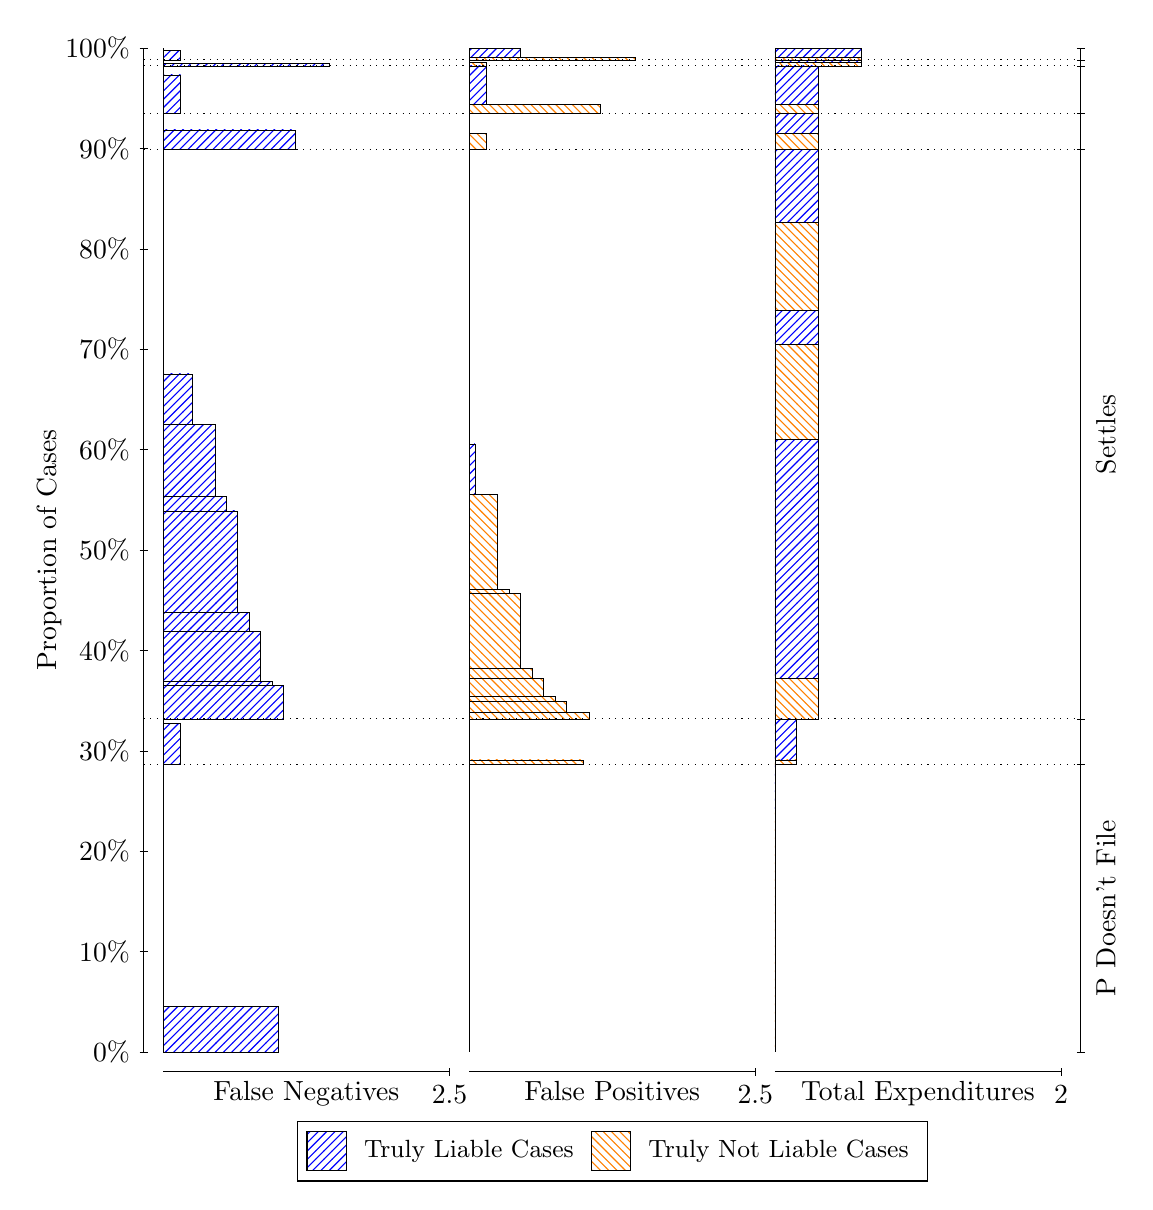
\begin{tikzpicture}
\draw[black, very thin] (1.5,1.75) -- (1.5,14.5);
\node[rotate=90, text=black, anchor=center] at (0.3, 8.125) {Proportion of Cases};
\draw[black, very thin] (1.45,1.75) -- (1.55,1.75);
\node[text=black, anchor=east] at (1.45, 1.75) {0\%};
\draw[black, very thin] (1.45,3.025) -- (1.55,3.025);
\node[text=black, anchor=east] at (1.45, 3.025) {10\%};
\draw[black, very thin] (1.45,4.3) -- (1.55,4.3);
\node[text=black, anchor=east] at (1.45, 4.3) {20\%};
\draw[black, very thin] (1.45,5.575) -- (1.55,5.575);
\node[text=black, anchor=east] at (1.45, 5.575) {30\%};
\draw[black, very thin] (1.45,6.85) -- (1.55,6.85);
\node[text=black, anchor=east] at (1.45, 6.85) {40\%};
\draw[black, very thin] (1.45,8.125) -- (1.55,8.125);
\node[text=black, anchor=east] at (1.45, 8.125) {50\%};
\draw[black, very thin] (1.45,9.4) -- (1.55,9.4);
\node[text=black, anchor=east] at (1.45, 9.4) {60\%};
\draw[black, very thin] (1.45,10.675) -- (1.55,10.675);
\node[text=black, anchor=east] at (1.45, 10.675) {70\%};
\draw[black, very thin] (1.45,11.95) -- (1.55,11.95);
\node[text=black, anchor=east] at (1.45, 11.95) {80\%};
\draw[black, very thin] (1.45,13.225) -- (1.55,13.225);
\node[text=black, anchor=east] at (1.45, 13.225) {90\%};
\draw[black, very thin] (1.45,14.5) -- (1.55,14.5);
\node[text=black, anchor=east] at (1.45, 14.5) {100\%};

\draw[black, very thin] (13.4,1.75) -- (13.4,14.5);
\draw[black, very thin] (13.35,1.75) -- (13.45,1.75);
\node[anchor=west] at (13.35, 1.75) {};
\draw[black, very thin] (13.35,5.4021) -- (13.45,5.4021);
\node[anchor=west] at (13.35, 5.4021) {};
\draw[black, very thin] (13.35,5.9813) -- (13.45,5.9813);
\node[anchor=west] at (13.35, 5.9813) {};
\draw[black, very thin] (13.35,13.211) -- (13.45,13.211);
\node[anchor=west] at (13.35, 13.211) {};
\draw[black, very thin] (13.35,13.67) -- (13.45,13.67);
\node[anchor=west] at (13.35, 13.67) {};
\draw[black, very thin] (13.35,14.274) -- (13.45,14.274);
\node[anchor=west] at (13.35, 14.274) {};
\draw[black, very thin] (13.35,14.349) -- (13.45,14.349);
\node[anchor=west] at (13.35, 14.349) {};
\draw[black, very thin] (13.35,14.5) -- (13.45,14.5);
\node[anchor=west] at (13.35, 14.5) {};

\draw[black, very thin, pattern color=blue, pattern=north east lines] (1.75,1.75) rectangle (3.2033,2.3321);
\draw[black, very thin, pattern color=orange, pattern=north west lines] (1.75,2.3321) rectangle (1.75,5.4021);
\draw[black, very thin, pattern color=blue, pattern=north east lines] (1.75,5.4021) rectangle (1.968,5.9236);
\draw[black, very thin, pattern color=orange, pattern=north west lines] (1.75,5.9236) rectangle (1.75,5.9813);
\draw[black, very thin, pattern color=blue, pattern=north east lines] (1.75,5.9813) rectangle (3.276,6.408);
\draw[black, very thin, pattern color=blue, pattern=north east lines] (1.75,6.408) rectangle (3.1307,6.4579);
\draw[black, very thin, pattern color=blue, pattern=north east lines] (1.75,6.4579) rectangle (2.9853,7.0938);
\draw[black, very thin, pattern color=blue, pattern=north east lines] (1.75,7.0938) rectangle (2.84,7.3314);
\draw[black, very thin, pattern color=blue, pattern=north east lines] (1.75,7.3314) rectangle (2.6947,8.6223);
\draw[black, very thin, pattern color=blue, pattern=north east lines] (1.75,8.6223) rectangle (2.5493,8.8057);
\draw[black, very thin, pattern color=blue, pattern=north east lines] (1.75,8.8057) rectangle (2.404,9.7209);
\draw[black, very thin, pattern color=blue, pattern=north east lines] (1.75,9.7209) rectangle (2.1133,10.363);
\draw[black, very thin, pattern color=orange, pattern=north west lines] (1.75,10.363) rectangle (1.75,13.211);
\draw[black, very thin, pattern color=blue, pattern=north east lines] (1.75,13.211) rectangle (3.4213,13.461);
\draw[black, very thin, pattern color=orange, pattern=north west lines] (1.75,13.461) rectangle (1.75,13.67);
\draw[black, very thin, pattern color=blue, pattern=north east lines] (1.75,13.67) rectangle (1.968,14.159);
\draw[black, very thin, pattern color=orange, pattern=north west lines] (1.75,14.159) rectangle (1.75,14.274);
\draw[black, very thin, pattern color=blue, pattern=north east lines] (1.75,14.274) rectangle (3.8573,14.308);
\draw[black, very thin, pattern color=orange, pattern=north west lines] (1.75,14.308) rectangle (1.75,14.349);
\draw[black, very thin, pattern color=blue, pattern=north east lines] (1.75,14.349) rectangle (1.968,14.466);
\draw[black, very thin, pattern color=orange, pattern=north west lines] (1.75,14.466) rectangle (1.75,14.5);
\draw[black, very thin, pattern color=orange, pattern=north west lines] (5.6333,1.75) rectangle (5.6333,4.82);
\draw[black, very thin, pattern color=blue, pattern=north east lines] (5.6333,4.82) rectangle (5.6333,5.4021);
\draw[black, very thin, pattern color=orange, pattern=north west lines] (5.6333,5.4021) rectangle (7.0867,5.4598);
\draw[black, very thin, pattern color=blue, pattern=north east lines] (5.6333,5.4598) rectangle (5.6333,5.9813);
\draw[black, very thin, pattern color=orange, pattern=north west lines] (5.6333,5.9813) rectangle (7.1593,6.0674);
\draw[black, very thin, pattern color=orange, pattern=north west lines] (5.6333,6.0674) rectangle (6.8687,6.1994);
\draw[black, very thin, pattern color=orange, pattern=north west lines] (5.6333,6.1994) rectangle (6.7233,6.265);
\draw[black, very thin, pattern color=orange, pattern=north west lines] (5.6333,6.265) rectangle (6.578,6.4983);
\draw[black, very thin, pattern color=orange, pattern=north west lines] (5.6333,6.4983) rectangle (6.4327,6.6258);
\draw[black, very thin, pattern color=orange, pattern=north west lines] (5.6333,6.6258) rectangle (6.2873,7.5762);
\draw[black, very thin, pattern color=orange, pattern=north west lines] (5.6333,7.5762) rectangle (6.142,7.6225);
\draw[black, very thin, pattern color=orange, pattern=north west lines] (5.6333,7.6225) rectangle (5.9967,8.8291);
\draw[black, very thin, pattern color=blue, pattern=north east lines] (5.6333,8.8291) rectangle (5.706,9.4716);
\draw[black, very thin, pattern color=blue, pattern=north east lines] (5.6333,9.4716) rectangle (5.6333,13.211);
\draw[black, very thin, pattern color=orange, pattern=north west lines] (5.6333,13.211) rectangle (5.8513,13.42);
\draw[black, very thin, pattern color=blue, pattern=north east lines] (5.6333,13.42) rectangle (5.6333,13.67);
\draw[black, very thin, pattern color=orange, pattern=north west lines] (5.6333,13.67) rectangle (7.3047,13.785);
\draw[black, very thin, pattern color=blue, pattern=north east lines] (5.6333,13.785) rectangle (5.8513,14.274);
\draw[black, very thin, pattern color=orange, pattern=north west lines] (5.6333,14.274) rectangle (5.8513,14.315);
\draw[black, very thin, pattern color=blue, pattern=north east lines] (5.6333,14.315) rectangle (5.6333,14.349);
\draw[black, very thin, pattern color=orange, pattern=north west lines] (5.6333,14.349) rectangle (7.7407,14.383);
\draw[black, very thin, pattern color=blue, pattern=north east lines] (5.6333,14.383) rectangle (6.2873,14.5);
\draw[black, very thin, pattern color=orange, pattern=north west lines] (9.5167,1.75) rectangle (9.5167,4.82);
\draw[black, very thin, pattern color=blue, pattern=north east lines] (9.5167,4.82) rectangle (9.5167,5.4021);
\draw[black, very thin, pattern color=orange, pattern=north west lines] (9.5167,5.4021) rectangle (9.7892,5.4598);
\draw[black, very thin, pattern color=blue, pattern=north east lines] (9.5167,5.4598) rectangle (9.7892,5.9813);
\draw[black, very thin, pattern color=orange, pattern=north west lines] (9.5167,5.9813) rectangle (10.062,6.4983);
\draw[black, very thin, pattern color=blue, pattern=north east lines] (9.5167,6.4983) rectangle (10.062,9.5303);
\draw[black, very thin, pattern color=orange, pattern=north west lines] (9.5167,9.5303) rectangle (10.062,10.737);
\draw[black, very thin, pattern color=blue, pattern=north east lines] (9.5167,10.737) rectangle (10.062,11.164);
\draw[black, very thin, pattern color=orange, pattern=north west lines] (9.5167,11.164) rectangle (10.062,12.288);
\draw[black, very thin, pattern color=blue, pattern=north east lines] (9.5167,12.288) rectangle (10.062,13.211);
\draw[black, very thin, pattern color=orange, pattern=north west lines] (9.5167,13.211) rectangle (10.062,13.42);
\draw[black, very thin, pattern color=blue, pattern=north east lines] (9.5167,13.42) rectangle (10.062,13.67);
\draw[black, very thin, pattern color=orange, pattern=north west lines] (9.5167,13.67) rectangle (10.062,13.785);
\draw[black, very thin, pattern color=blue, pattern=north east lines] (9.5167,13.785) rectangle (10.062,14.274);
\draw[black, very thin, pattern color=orange, pattern=north west lines] (9.5167,14.274) rectangle (10.607,14.315);
\draw[black, very thin, pattern color=blue, pattern=north east lines] (9.5167,14.315) rectangle (10.607,14.349);
\draw[black, very thin, pattern color=orange, pattern=north west lines] (9.5167,14.349) rectangle (10.607,14.383);
\draw[black, very thin, pattern color=blue, pattern=north east lines] (9.5167,14.383) rectangle (10.607,14.5);
\draw[black, dotted] (1.5,5.4021) -- (13.4,5.4021);
\draw[black, dotted] (1.5,5.9813) -- (13.4,5.9813);
\draw[black, dotted] (1.5,13.211) -- (13.4,13.211);
\draw[black, dotted] (1.5,13.67) -- (13.4,13.67);
\draw[black, dotted] (1.5,14.274) -- (13.4,14.274);
\draw[black, dotted] (1.5,14.349) -- (13.4,14.349);
\draw[black, very thin] (1.75,1.5) -- (5.3833,1.5);
\node[text=black, anchor=north] at (3.5667, 1.5) {False Negatives};
\draw[black, very thin] (5.3833,1.45) -- (5.3833,1.55);
\node[text=black, anchor=north] at (5.3833, 1.45) {2.5};

\draw[black, very thin] (5.6333,1.5) -- (9.2667,1.5);
\node[text=black, anchor=north] at (7.45, 1.5) {False Positives};
\draw[black, very thin] (9.2667,1.45) -- (9.2667,1.55);
\node[text=black, anchor=north] at (9.2667, 1.45) {2.5};

\draw[black, very thin] (9.5167,1.5) -- (13.15,1.5);
\node[text=black, anchor=north] at (11.333, 1.5) {Total Expenditures};
\draw[black, very thin] (13.15,1.45) -- (13.15,1.55);
\node[text=black, anchor=north] at (13.15, 1.45) {2};

\node[text=black, centered, rotate=90] at (13.72, 3.576) {P Doesn't File};

\node[text=black, centered, rotate=90] at (13.72, 9.5963) {Settles};





\draw (7.449999999999999,1.5) node[draw=none] (baseCoordinate) {};
\begin{scope}[align=center]
        \matrix[scale=0.5, draw=black, below=0.5cm of baseCoordinate, nodes={draw}, column sep=0.1cm]{
            \node[rectangle, draw, minimum width=0.5cm, minimum height=0.5cm, pattern color=blue, pattern=north east lines] {}; &
            \node[draw=none, font=\small, text=black] (B) {Truly Liable Cases}; &
            \node[rectangle, draw, minimum width=0.5cm, minimum height=0.5cm, pattern color=orange, pattern=north west lines] {}; &
            \node[draw=none, font=\small, text=black] (B) {Truly Not Liable Cases}; \\
            };
\end{scope}

\end{tikzpicture}
\end{document}